\label{chapter:background}

\section{Summarization}

\subsection{Definition} \label{sec:definition}

As described by the author in \cite{lloret_text_2008}, a summary is a way of providing a large part of the information contained in one or more original passages, using at most half of the text. Summaries can be grouped into one of the two following categories:

\begin{itemize}[nolistsep]
\item An \textit{extract} is made up of sentences which are copied word-for-word.
\item An \textit{abstract} is a rewriting of the original text's content in a more concise form.
\end{itemize}

\mbox{}

A different way to group summaries is the following:

\begin{itemize}[nolistsep]
\item \textit{Generic} summaries do not try and focus on anything in particular, they simply aim to recount the most important features.
\item \textit{Focused} (or \textit{query-driven}) summaries, on the other hand, require a user-input, which specifies the focus of the summary. For this project, we may want to introduce a bias to our learning program, so that we end up with a summary which meets a certain number of criteria. For instance, we might want it to ensure it captures at least one action verb from the original passage.
\end{itemize}

\mbox{}

Yet another way \cite{radev_introduction_2002} is shown below, with examples given in Figure \ref{fig:indicative_informative_summaries}:

\begin{itemize}[nolistsep]
\item \textit{Indicative} summaries give the overall impression of a text, but without conveying any details.
\item \textit{Informative} summaries, on the other hand, take the content from an original document and give a shortened version of it.
\end{itemize}

\begin{figure}[H]\
\begin{subfigure}{\textwidth}
\begin{displayquote}
It’s going to be windy across the western half of the UK, with gusts reaching 60 to 70mph along Irish Sea coastlines, the west of Scotland and perhaps some English Channel coasts. Those in affected areas are advised to take extra care when driving on bridges or high open roads. Flood warnings were issued on Sunday for two areas – Keswick campsite in Cumbria and a stretch along the River Nene east of Peterborough.
\end{displayquote}
\caption{\textit{Indicative} summary}
\vspace{\baselineskip}
\end{subfigure}
\begin{subfigure}{\textwidth}
\begin{displayquote}
Yellow warnings of strong winds were put in place for parts of the UK. These very strong winds are likely to cause travel disruption, so those in affected areas are advised to take extra care when driving on exposed routes. In addition, heavy rain is expected in parts of the country, which could cause local flooding.
\caption{\textit{Informative} summary}
\end{displayquote}
\end{subfigure}
\caption{Example of \textit{indicative} and \textit{informative} summaries for a \href{https://www.theguardian.com/uk-news/2020/jan/12/storm-brendan-gales-forecast-uk}{news article}}
\label{fig:indicative_informative_summaries}
\end{figure}

\section{Syntactic Parsing}

Given a text, \textit{syntactic parsing} \cite{noauthor_syntactic_nodate} describes the process of tokenization, whereby the grammatical link between parts of speech is established.
Two of the most prominent syntactic parsers are \textbf{\href{https://corenlp.run}{CoreNLP}} (developed by Stanford) and \textbf{\href{https://spacy.io}{spaCy}}.

This tokenization can then be visualized in the form of a tree, which makes it possible to identify different parts of speech, such as nouns, verbs and adjectives. An example is shown in Table \ref{table:basic_sentence} for both of the mentioned parsers. Appendix \ref{appendix:pos} shows how to interpret position of speech (POS) tags.

\begin{table}[H]
\centering
\begin{tabular}{@{}ll@{}}
\toprule
\textbf{CoreNLP} & 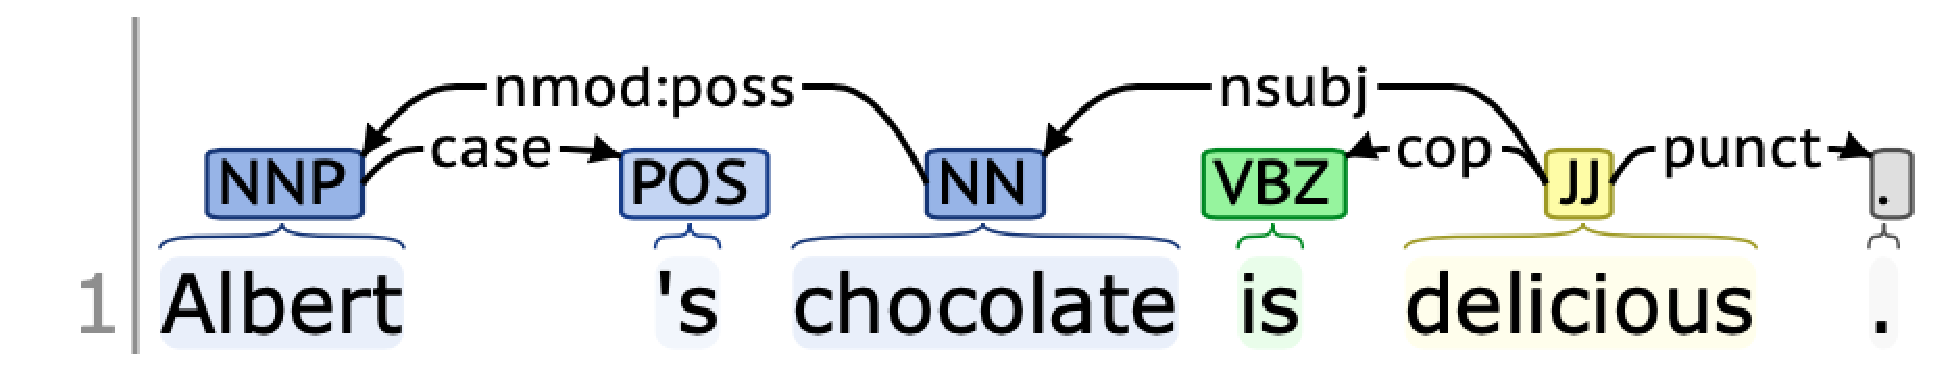
\includegraphics[width=0.75\textwidth]{basic_sentence_core_nlp.eps} \\ \midrule
\textbf{spaCy} & 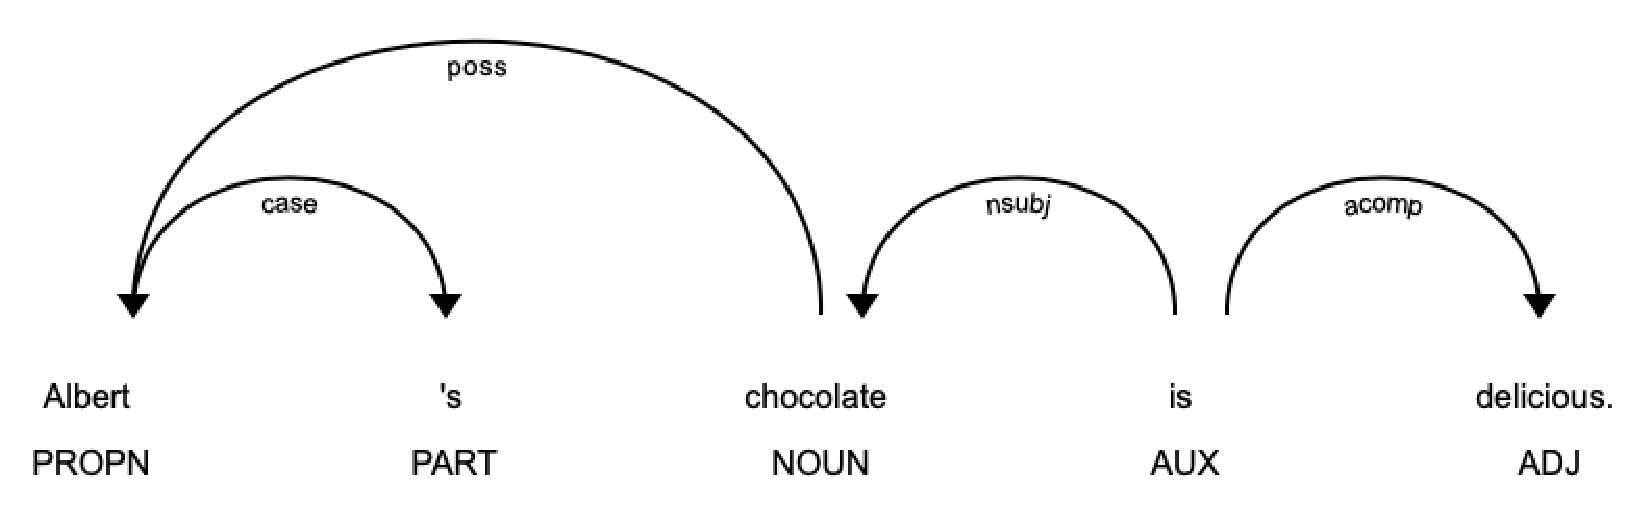
\includegraphics[width=0.85\textwidth]{basic_sentence_spacy.eps}  \\ \bottomrule
\end{tabular}
\caption{Semantic parsing example for a basic sentence}
\label{table:basic_sentence}
\end{table}

However, the English language can often be ambiguous and highly context-dependent, meaning that multiple \textit{parse trees} for the same sentence could emerge. Consider the following two sentences \cite{noauthor_studying_nodate}:
\begin{displayquote}
He fed her cat food. \\
I saw a man on a hill with a telescope.
\end{displayquote}
As shown in Table \ref{table:ambiguous_sentence}, both parsers interpret the meaning of the first example sentence as a person who feeds their ``cat food", which, in addition of not being very logical, is also grammatically incorrect as the genders do not match. Unfortunately, computers are generally not very good at context-based inference, something to take into account for this research project.

Therefore accuracy is very important for \textit{syntactic parsing} \cite{gomez-rodriguez_how_2019}.

\begin{table}[H]
\centering
\begin{tabular}{@{}ll@{}}
\toprule
\textbf{CoreNLP} & 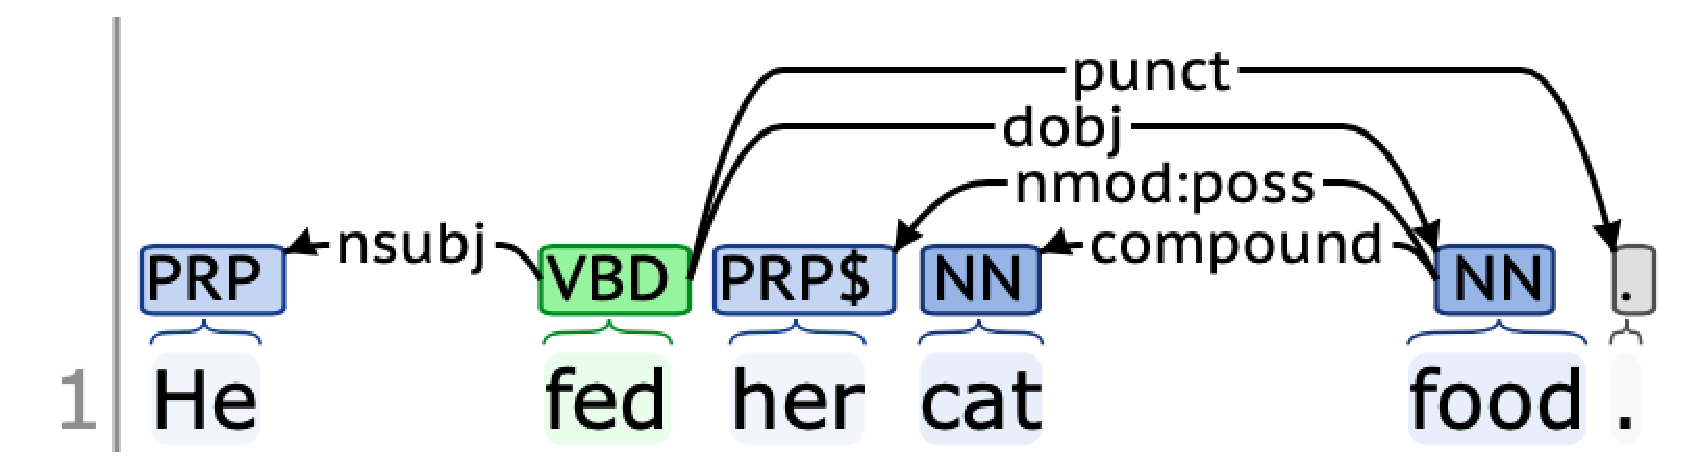
\includegraphics[width=0.75\textwidth]{ambiguous_sentence_core_nlp.eps} \\ \midrule
\textbf{spaCy} & 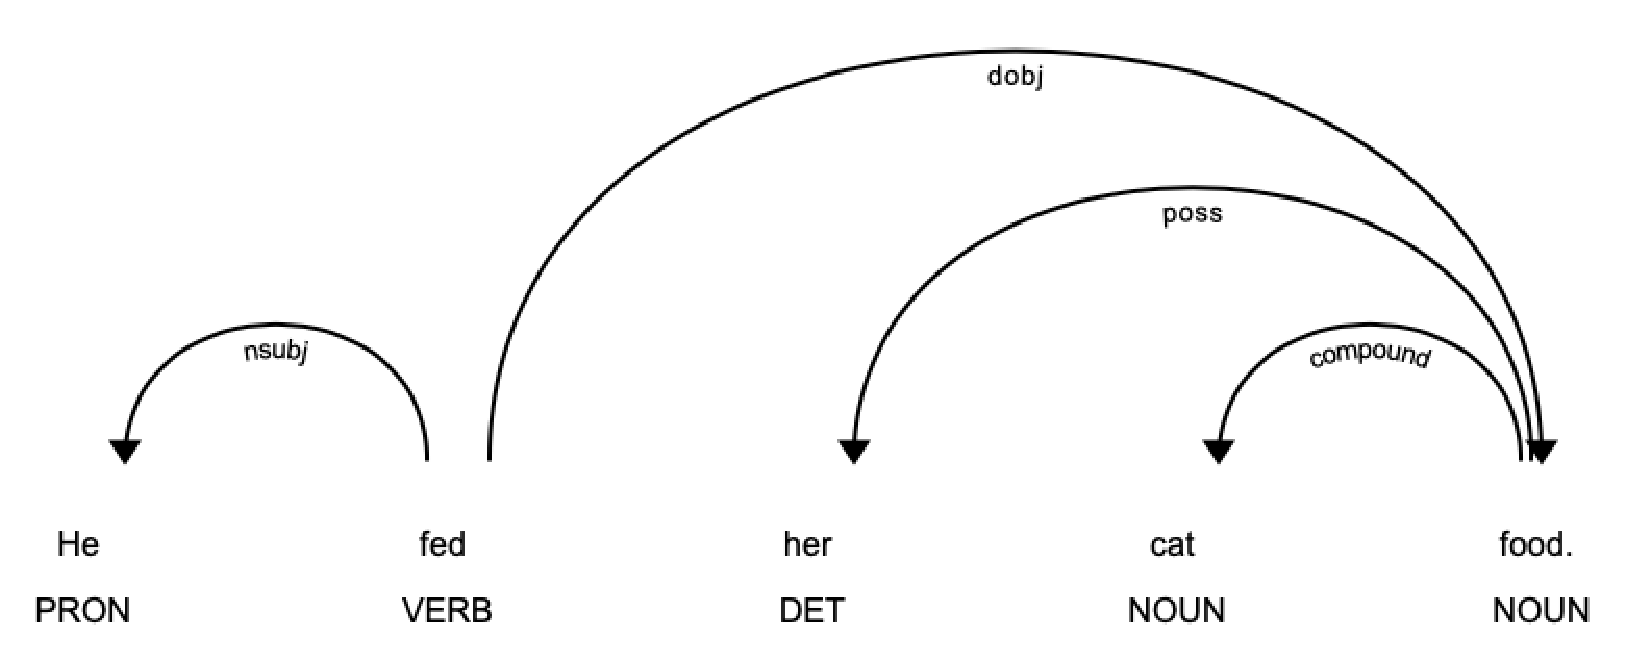
\includegraphics[width=0.85\textwidth]{ambiguous_sentence_spacy.eps}  \\ \bottomrule
\end{tabular}
\caption{Semantic parsing example for an ambiguous sentence}
\label{table:ambiguous_sentence}
\end{table}

\section{Logic Programming}

\begin{definition}[Term \cite{kowalski_predicate_1974}]
A \textit{term} is either a \textit{variable} $x,y,z,...$ or an expression $f(t_1,t_2,...,t_k)$, where $f$ is a k-ary \textit{function symbol} and the $t_i$ are \textit{terms}. A \textit{constant} is a 0-ary \textit{function symbol}.
\end{definition}

\begin{definition}[Atom \cite{kowalski_predicate_1974}]
An \textit{atomic formula} (or \textit{atom}) has the form $P(t_1,t_2,...,t_k)$, where $P$ is a k-ary predicate (boolean function) symbol and the $t_i$ are terms.
\end{definition}

\subsection{Answer Set Programming}

Once we have parsed a text, the next step is to convert this into an answer set program (ASP).

ASP is a declarative first-order (predicate) logic language whose aim is to solve hard search problems \cite{lifschitz_what_nodate}. It is built upon the idea of stable model (answer set) semantics, returns answer sets when asked for the solution to a problem.

In ASP, a \textit{literal} is an \textit{atom} \textit{a} or its negation \textit{not a} (we call this negation as a failure). ASP programs are composed of a set of \textit{normal rules}, whose head is a single \textit{atom} and body is a conjunction of \textit{literals} \cite{law_representing_2019}.
\begin{equation}
h \leftarrow b_1, b_2, ..., b_k, \text{not}\ b_{k+1}, ..., \text{not}\ b_m.
\end{equation}

If the body is empty ($k = m = 0$) then a rule is called a \textit{fact}. We can also have \textit{constraints}, which are like \textit{normal rules} except that the head is empty. These prevent any answer sets from both including $b_1, b_2, ..., b_k$ and excluding $b_{k+1}, ..., b_m$.

\begin{definition}[Safety \cite{law_representing_2019}]
A variable in a rule is said to be \textit{safe} if it occurs in at least one positive \textit{literal} (i.e. the $b_i$s in the above rule) in the body of the rule.
\end{definition}

\begin{definition}[Herbrand Base \cite{law_representing_2019}]
The \textit{Herbrand base} of a program P, denoted $HB_P$, is the set of variable-free (\textit{ground}) \textit{atoms} that can be formed from predicates and \textit{constants} in P . The subsets of $HB_P$ are called the (Herbrand) \textit{interpretations} of P.
\end{definition}

\begin{definition}[Satisfiability \cite{law_representing_2019}] 
\label{def:satisfiability}
Given a set $A$, a \textit{ground normal rule} of P is \textit{satisfied} if the head is in $A$ when all positive \textit{atoms} and none of the negated \textit{atoms} of the body are in $A$, that is when the body is \textit{satisfied}. A \textit{ground constraint} is \textit{satisfied} when the body is not \textit{satisfied}.
\end{definition}

\begin{definition}[Reduct \cite{law_representing_2019}]
Given a program P and an \textit{Herbrand interpretation} $I \subseteq HB_P$, the \textit{reduct} $P^I$ is constructed from the grounding of P in three steps:
\begin{enumerate}[nolistsep]
\item Remove rules whose bodies contain the negation of an atom in I.
\item Remove all negative \textit{literals} from the remaining rules.
\item Replace the head of any constraint with $\bot$ (where $\bot \notin HB_P$).
\end{enumerate}
For example, the \textit{reduct} of the program $\{a \leftarrow \text{not}\ b, c.\quad d \leftarrow \text{not}\ c.\}$ with respect to $I=\{b\}$ is $\{d.\}$.
\end{definition}

\begin{definition}[Minimal Model]
We say that $I$ is a (Herbrand) \textit{model} when $I$ \textit{satisfies} all the rules in the program P. It is a \textit{minimal model} if there exists no smaller \textit{model} than $I$.
\end{definition}

\begin{definition}[Answer Set \cite{law_representing_2019}]
Any $I \subseteq HB_P$ is an \textit{answer set} of P if it is equal to the \textit{minimal model}  of the \textit{reduct} $P^I$. We will denote the set of \textit{answer sets} of a program P with $AS(P)$. 
\end{definition}

%A \textit{constraint} has therefore the effect of eliminating all \textit{answer sets} of P that \textit{satisfy} the body of the \textit{constraint}. \cite{law_representing_2019}.

\subsection{Context-Free Grammars}

In order to discuss answer set grammars (ASGs), we must first define \textit{context-free grammars} (CFGs) and \textit{parse trees}. An example for these is shown in Figure \ref{fig:cfg_parse_tree_example}.

\begin{definition}[Context-Free Grammar \cite{scheinberg_note_1960}]
A CFG is a finite set G of ``rewriting rules" $\alpha \to \beta$, where $\alpha$ is a single symbol and $\beta$ is a finite string of symbols from a finite alphabet (vocabulary) V. V contains precisely the symbols appearing in these rules plus the ``boundary" symbol $\epsilon$, which does not appear in these rules. Rules of the form $\alpha \to \alpha$ (which have no effect) are not allowed.
\end{definition}

%\begin{definition}[Context-Free Grammar \cite{law_representing_2019}]
%A \textit{context-free grammar} $G_{CF}$ is a tuple $\langle G_N,G_T,G_{PR},G_S \rangle$ where $G_N$ is a (finite) set of non-terminal nodes, $G_T$ is a (finite) set, disjoint from $G_N$, of terminal nodes, $G_{PR}$ is a set of production rules of the form $n_0 \to n_1 ... n_k$, where $n_0 \in G_N$ and each $n_i \in G_N \cup G_T$. $G_S \in G_N$ is the start node of $G_{CF}$.
%\end{definition}

\begin{definition}[Parse Tree \cite{law_representing_2019}]
Let $GCF$ be a CFG. A \textit{parse tree} $PT$ of $GCF$ for a given string consists of a node $node(PT)$, a list of \textit{parse trees}, called \textit{children} and denoted $children(PT)$, and a rule $rule(PT)$, such that:
\begin{enumerate}[nolistsep]
\item If $node(PT)$ is a terminal node, then $children(PT)$ is empty.
\item If $node(PT)$ is non-terminal, then $rule(PT)$ is of the form $node(PT) \to n_1 ... n_k$ where each $n_i$ is equal to $node(children(PT)[i])$ and $|children(PT)| = k$.
\end{enumerate}
%For any \textit{parse tree} $PT$ we define $str(PT)$ as: $node(PT)$ if $node(PT) \in G_T$; and $str(PT_1) ... str(PT_n)$ otherwise (where $[PT_1, ..., PT_n] = children(PT))$. A \textit{parse tree} $PT$ of $GCF$ is a \textit{parse tree} for a string $s$ if $node(PT) = GS$ and $s = str(PT)$.
\end{definition}

\begin{definition}[Trace \cite{law_representing_2019}]
We can represent each node n in a \textit{parse tree} by its \textit{trace}, $trace(n)$, through the tree. The \textit{trace} of the root is the empty list \texttt{[]}; the i\textsuperscript{th} child of the root is \texttt{[i]}; the j\textsuperscript{th} child of the i\textsuperscript{th} child of the root is \texttt{[i, j]}, and so on.
\end{definition}

\begin{figure}[H]
\begin{subfigure}{0.3\textwidth}
\texttt{1: start -> as "b" \\ 2: as -> "a" as \\ 3: as ->\\}
\caption{CFG for \texttt{a\textsuperscript{i}b}}
\end{subfigure}
\begin{subfigure}{0.34\textwidth}
\centering
\begin{table}[H]
\begin{tabular}{@{}ccc@{}}
\toprule
\textbf{$trace(n)$} & \textbf{$node(n)$} \\ \midrule
\texttt{[]} & \texttt{start} \\
\texttt{[1]} & \texttt{as} \\
\texttt{[1,1]} & \texttt{a} \\
\texttt{[1,2]} & \texttt{as} \\
\texttt{[1,2,1]} & \texttt{a} \\
\texttt{[1,2,2]} & \texttt{as} \\
\texttt{[2]} & \texttt{b} \\ \bottomrule
\end{tabular}
\end{table}
\caption{\textit{Parse tree} table for \texttt{aab}}
\end{subfigure}
\begin{subfigure}{0.34\textwidth}
\centering
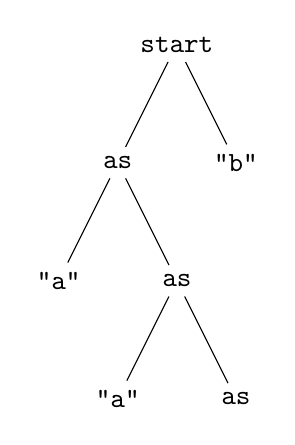
\begin{tikzpicture}
\node {\texttt{start}}
  child {node {\texttt{as}}
    child {node {\texttt{"a"}}}
    child {node {\texttt{as}}
      child {node {\texttt{"a"}}}
      child {node {\texttt{as}}}}}
  child {node {\texttt{"b"}}};
\end{tikzpicture}
\caption{\textit{Parse tree} graph for \texttt{aab}}
\end{subfigure}
\caption{Example of a CFG and its \textit{parse tree}}
\label{fig:cfg_parse_tree_example}
\end{figure}

\subsection{Answer Set Grammars}

ASGs are an extension of CFGs, whereby each production rule is \textit{annotated}. More specifically, $P$ can be a \textit{ground term}, such as in the \textit{annotated atom} \texttt{a(1)@2} (referring to the second child of this node). The example shown in Figure \ref{fig:asg_example} is a subset of the language \texttt{a\textsuperscript{i}b} captured by the CFG in Figure \ref{fig:cfg_parse_tree_example},  restricting it to the language \texttt{a\textsuperscript{n}} where $\texttt{n} \ge 2$ (the string contains at least two as).

\begin{definition}[Answer Set Grammar \cite{law_representing_2019}]
 An \textit{annotated} production rule is of the form $n_0 \to n_1 ... n_k\ P$ where $n_0 \to n_1 ... n_k$ is an ordinary CFG production rule and $P$ is an \textit{annotated} ASP program, where every \textit{annotation} is an integer from $1$ to $k$.
\end{definition}

\begin{figure}[H]
\texttt{1: start -> as "b" \{ :- size(X)@1, X < 1. \} \\
           2: as -> "a" as \space\space\space\{ size(X+1) :- size(X)@2. \} \\
           3: as -> \space\space\space\space\space\space\space\space\space\space\{ size(0). \} \\}\\
* Intuitively, \texttt{size} represents the length of the current string.
\caption{Example of an ASG}
\label{fig:asg_example}
\end{figure}

\begin{definition}[Parse Tree Program \cite{law_representing_2019}]
Let G be an ASG and PT be a \textit{parse tree}. $G[PT]$ is the program $\{\ rule(n)@trace(n)\ |\ n \in PT\ \}$, where for any production rule $n_0 \to n_1...n_k\ P$, and any trace $t$, $PR@t$ is the program constructed by replacing all annotated atoms $a@i$ with the atom $a@t++[i]$ and all \textit{unannotated atoms} $a$ with the atom $a@t$.
\end{definition}

\begin{definition}[Conforming Parse Tree \cite{law_representing_2019}]
Given a string $str$ of terminal nodes, we say that $str \in \mathcal{L}(G)$ ($str$ \textit{conforms} to the language of G) if and only if there exists a parse tree PT of G for $str$ such that the program $G[PT]$ is \textit{satisfiable}. For such a PT, every single rule in the language must be satisfied (see Definition \ref{def:satisfiability}).
\end{definition}

As shown in Figure \ref{fig:asg_tree_program_example}, $\texttt{aab} \in \mathcal{L}(G)$, and the corresponding program has a single answer set $\{size(0)@[1,2,2],\ size(1)@[1,2],\ size(2)@[1]\}$. From this example, it is easy to see how the corresponding program would be \textit{unsatisfiable} for the string \texttt{ab}.

\begin{figure}[H]
\centering
\texttt{:- size(X)@[1], X < 1. \\
           size(X+1)@[1] :- size(X)@[1,2]. \\
           size(X+1)@[1,2] :- size(X)@[1,2,2]. \\
           size(0)@[1,2,2].}
\caption{$G[PT]$ for the \textit{parse tree} and ASG from the examples above}
\label{fig:asg_tree_program_example}
\end{figure}

\subsection{Learning Answer Set Grammars}

Given an incomplete ASG, it is possible to learn the complete grammar by induction (which uses \href{http://www.ilasp.com}{ILASP}), as long as we provide some \textit{positive examples} (strings which should conform to the language), \textit{negative examples}  (strings which must not), as well as a \textit{hypothesis space} and usually some \textit{background} information. Note that the \textit{background} is only used for ``global" knowledge, such as defining what is a number, or how to increment one. \cite{law_representing_2019}

In such an \textit{inductive learning program} (ILP) task, we have a \textit{hypothesis space} in the form of \textit{mode declarations}, defining the format of the heads (written \texttt{\#modeh}) and bodies (written \texttt{\#modeb}) of rules which can be learned. It is also possible to restrict the scope of a particular \textit{mode declaration} by specifying a list of rule numbers at the end. Note that there are two forms of body \textit{mode declarations}: \texttt{\#modeba} is used for predicates that accept an $@$ \textit{annotation}, and \texttt{\#modebb} is intended for those without (which are defined in \texttt{\#background}). An example is shown in Figure \ref{fig:asg_ilp_example}.

\begin{figure}[H]
\centering
\begin{subfigure}{0.55\textwidth}
\texttt{start -> as bs \{\} \\
as -> "a" as \{\} | \{\} \\
bs -> "b" bs \{\} | \{\} \\
\newline
+ [] \\
+ ["a", "b"] \\
+ ["a", "a", "b", "b"] \\
- ["a"] \\
- ["b"] \\
- ["a", "a"] \\
- ["b", "b"] \\
- ["a", "a", "b"] \\
- ["a", "b", "b"] \\
\newline
\#background \{ \\
num(0). num(1). num(2). num(3). \\
inc(X,X+1) :- num(X), num(X+1). \} \\
\newline
\#modeh(size(var(num))):[2,3,4,5]. \\
\#modeh(size(0)):[2,3,4,5]. \\
\#modeba(size(var(num))). \\}
\caption{Input incomplete program}
\end{subfigure}
\begin{subfigure}{0.44\textwidth}
\texttt{start -> as bs \{ \\
\phantom{ }:- not size(X)@2, size(X)@1. \\
\} \\
\newline
as -> "a" as \{ \\
\phantom{ }size(X+1) :- size(X)@2. \\
\} \\
\newline
as -> \{ \\
\phantom{ }size(0). \\
\} \\
\newline
bs -> "b" bs \{ \\
\phantom{ }size(X+1) :- size(X)@2. \\
\} \\
\newline
bs -> \{ \\
\phantom{ }size(0). \\
\}} \\
\caption{Output learned program}
\end{subfigure}
\newline
\newline
* Note: the symbol \texttt{|} indicates multiplicity of production rules.
\caption{Example of an ASG ILP task for the language \texttt{a\textsuperscript{n}b\textsuperscript{n}}}
\label{fig:asg_ilp_example}
\end{figure}